\documentclass[12pt,a4paper]{article}
\usepackage[utf8]{inputenc}
\usepackage[T1]{fontenc}
\usepackage[polish]{babel}
\usepackage{amsmath}
\usepackage{graphicx}
\usepackage{float}
\usepackage{geometry}
\geometry{margin=2.5cm}

\title{Sprawozdanie z laboratorium\\Algorytmy Metaheurystyczne -- Lista 2}
\author{Jakub Kogut}
\date{\today}

\begin{document}

\maketitle

\section{Wstęp Teoretyczny}
Niniejsze opracowanie zawiera analizę eksperymentalną oraz podsumowanie wyników uzyskanych przy użyciu dwóch zaawansowanych technik optymalizacji dyskretnej: Symulowanego Wyżarzania (Simulated Annealing) oraz Algorytmu Poszukiwania z Zabronieniami (Tabu Search). Obie metaheurystyki zostały zaadaptowane do rozwiązywania problemu komiwojażera (TSP).

Metoda symulowanego wyżarzania należy do grupy algorytmów stochastycznych i bazuje na symulacji procesów fizycznych towarzyszących krzepnięciu substancji krystalicznych. Kluczową rolę odgrywa tu zmienna temperatura, determinująca elastyczność algorytmu w akceptowaniu nowych stanów. Zezwolenie na przejście do gorszego rozwiązania z prawdopodobieństwem opisanym funkcją rozkładu Boltzmanna $e^{\frac{f(X)-f(X^{\prime})}{T}}$ zapobiega utknięciu w lokalnych ekstremach i pozwala na szeroką eksplorację przestrzeni stanów.

Algorytm Tabu Search opiera się na strategii przeszukiwania lokalnego opartego na pamięci. Zastosowanie krótkotrwałej struktury danych, zwanej listą tabu, uniemożliwia wykonywanie ruchów powrotnych do niedawno odwiedzonych punktów. Mechanizm ten eliminuje ryzyko wpadnięcia w cykle obliczeniowe i zmusza algorytm do opuszczenia lokalnych minimów w celu poszukiwania lepszych konfiguracji.

\section{Eksperymenty: Symulowane Wyżarzanie}
\subsection{Strojenie parametrów na instancjach testowych}
W ramach pierwszej części zadań zbadano wpływ konfiguracji temperatury początkowej oraz współczynnika chłodzenia na efektywność wyznaczania optymalnych tras. Badania zrealizowano dla zbiorów danych o zróżnicowanej wielkości.

\begin{figure}[H]
    \centering
    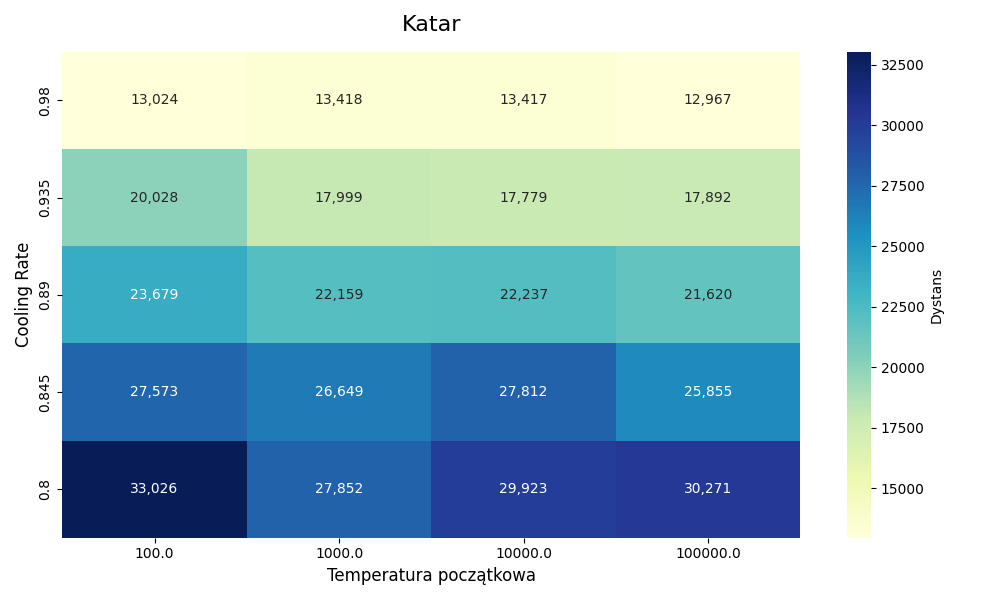
\includegraphics[width=0.8\textwidth]{../charts/Qatar1.png}
    \caption{Wpływ doboru temperatury startowej i tempa chłodzenia na wartość funkcji celu dla instancji Katar.}
    \label{fig:sa_qatar_eval}
\end{figure}

\begin{figure}[H]
    \centering
    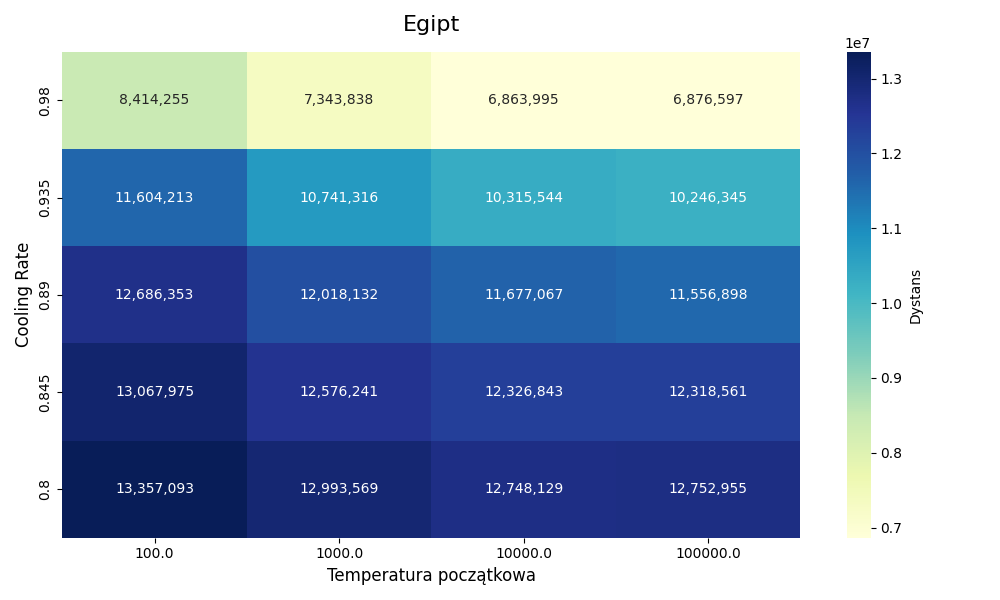
\includegraphics[width=0.8\textwidth]{../charts/Egipt1.png}
    \caption{Wykres zależności długości ścieżki od parametrów kontrolnych procesu wyżarzania (dane Egypt).}
    \label{fig:sa_egypt_eval}
\end{figure}

Dla dużej instancji problemu (Egipt) przeprowadzono serię 100 niezależnych uruchomień algorytmu, uzyskując następujące wskaźniki:
\begin{itemize}
    \item Najlepszy uzyskany wynik (minimum): 6 863 995
    \item Średnia długość trasy z całej serii: 11 124 295.95
\end{itemize}

\begin{figure}[H]
    \centering
    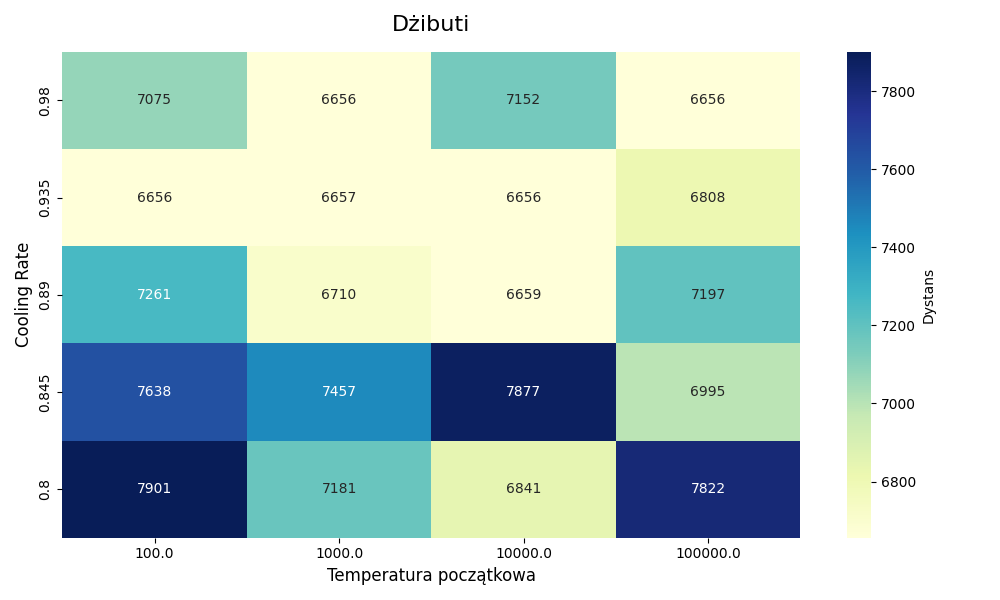
\includegraphics[width=0.8\textwidth]{../charts/Dzibuti1.png}
    \caption{Mapa cieplna przestrzeni rozwiązań w zależności od badanych parametrów SA dla instancji Djibouti.}
    \label{fig:sa_djibouti_eval}
\end{figure}

Zgromadzony materiał empiryczny zobrazowany na mapie cieplnej jednoznacznie wskazuje obszary parametrów gwarantujące zbieżność do globalnego optimum (osiągającego długość 6656). Wysoka temperatura początkowa połączona z relatywnie intensywnym tempem schładzania pozwala na skuteczną detekcję najlepszych tras bez generowania nadmiernego narzutu obliczeniowego.

\section{Eksperymenty: Tabu Search}
\subsection{Analiza wrażliwości parametrów sterujących}
Kolejny krok stanowiła parametryzacja i strojenie algorytmu Tabu Search. Analizie poddano dwa główne czynniki determinujące działanie algorytmu: długość kadencji ruchu na liście zabronień (\textit{tabu tenure}) oraz maksymalną dopuszczalną liczbę kroków bez poprawy rekordu (\textit{max stagnation}).

\begin{figure}[H]
    \centering
    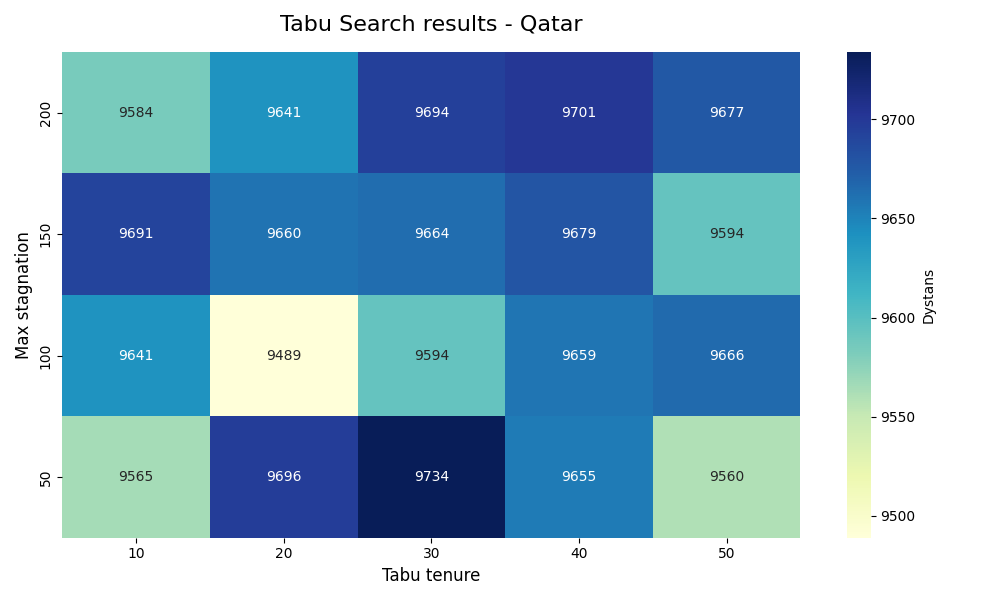
\includegraphics[width=0.8\textwidth]{../charts/Qatar2.png}
    \caption{Zależność końcowego dystansu od wielkości listy tabu oraz progu stagnacji w środowisku o zmiennych wynikach.}
    \label{fig:ts_var_analysis}
\end{figure}

Jak widać na powyższym wykresie, optymalne zachowanie algorytmu (skutkujące dystansem 9489) zanotowano przy zablokowaniu ruchów na 20 iteracji oraz limicie stagnacji ustawionym na 100 kroków. W dalszym toku badań zaobserwowano jednak specyficzne zachowanie, zilustrowane na kolejnym wykresie -- w pewnych warunkach modyfikacja parametrów w ogóle nie wpływa na ostateczną wartość funkcji celu.

\begin{figure}[H]
    \centering
    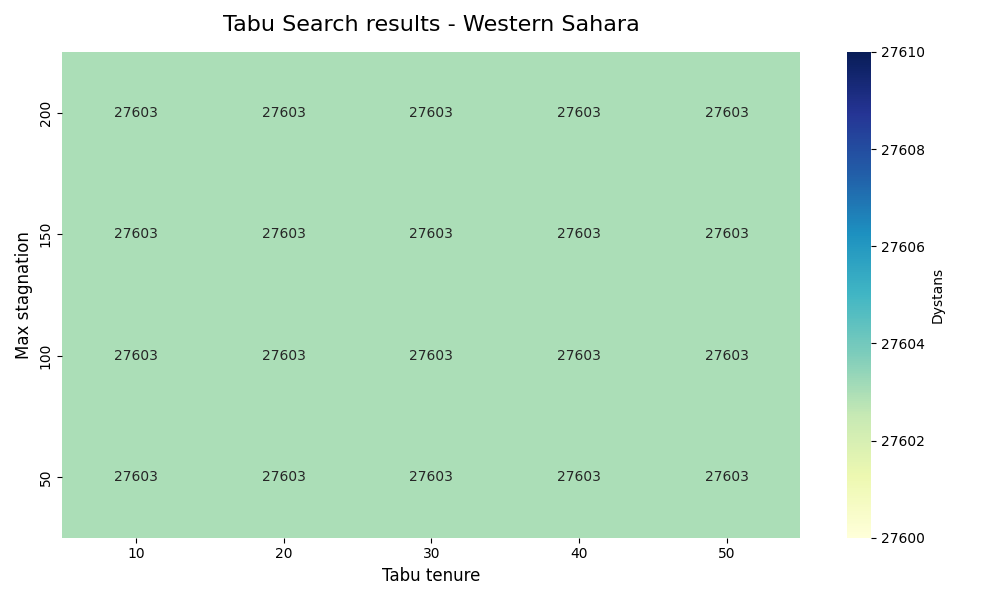
\includegraphics[width=0.8\textwidth]{../charts/WesternSahara.png}
    \caption{Wykres stabilności wyników algorytmu Tabu Search dla małej instancji problemu.}
    \label{fig:ts_const_analysis}
\end{figure}

Zjawisko uzyskiwania całkowicie homogenicznych (identycznych) rezultatów przez Tabu Search na małych zbiorach danych (np. Western Sahara) niezależnie od wybranych parametrów wynika bezpośrednio z następujących uwarunkowań:

\begin{enumerate}
    \item \textbf{Skala problemu a ukształtowanie przestrzeni (fitness landscape):} Bardzo mała liczba miast implikuje uproszczoną strukturę problemu. Przestrzeń poszukiwań jest na tyle niewielka, że algorytm bez przeszkód lokalizuje najlepszą trasę, która w tym przypadku stanowi rzeczywiste minimum globalne.
    
    \item \textbf{Systematyczna weryfikacja sąsiedztwa:} Implementacja algorytmu opiera się na pełnym, deterministycznym przeglądzie otoczenia o złożoności $\mathcal{O}(n^2)$ w każdej iteracji. Na małych grafach powoduje to nieuchronne i natychmiastowe skierowanie trajektorii poszukiwań do optymalnego punktu, niezależnie od wylosowanej konfiguracji początkowej.
    
    \item \textbf{Zredukowany wpływ nastaw algorytmu:} Ponieważ właściwa ścieżka odnajdywana jest na samym początku procesu, zwiększanie limitu \texttt{max\_stagnation} (np. z 50 do 200) nie polepsza rezultatu, a jedynie zmusza program do wykonywania jałowych pętli wokół znanego już rozwiązania. Z kolei wielkość listy \texttt{tabu\_tenure} przy tak małej liczbie miast jest w zupełności wystarczająca, by skutecznie zablokować powroty i zapętlenia.
\end{enumerate}

\textbf{Podsumowanie dla małych danych:} Na małych instancjach Tabu Search wyposażony w kompletny przegląd otoczenia wykazuje tak silną tendencję zbieżności, że jego działanie staje się niezmienne. Eksperymentowanie z parametrami kontrolnymi nie generuje w tym przypadku żadnych różnic w wynikach końcowych.

\section{Zestawienie Skuteczności i Wydajności Metod}
Końcowym etapem pracy było porównanie jakości oraz kosztów czasowych zaimplementowanych metaheurystyk z algorytmami stworzonymi w ramach poprzedniego bloku laboratoryjnego.

Algorytm Tabu Search charakteryzuje się wyższą dokładnością, lecz jest pod względem obliczeniowym sporo wolniejszy od algorytmu Symulowanego Wyżarzania. Wyższa precyzja oznacza w tym kontekście, że najlepsze znalezione przez Tabu Search rozwiązanie cechuje się lepszą wartością funkcji celu (krótszym dystansem całkowitym) niż rezultat wyznaczony przez SA.

Z kolei algorytm przeszukiwania lokalnego (Local Search) pochodzący z pierwszej listy zadań jest sporo dokładniejszy, a zarazem dużo wolniejszy od algorytmu Tabu Search.

\end{document}